\section{Results}
\label{sec:sherloc-results}


\subsection{RQ1 - Effectiveness}
%Table~\ref{tab:RQ1} shows the evaluation results for each formula.
%Overall, we observe that Dstar yields the worst results both in terms of accuracy and wasted effort. Out of the 38 analysed flaky classes, Dstar ranks 18 in the top 10, \ie 47\% of the classes. Dstar also results in the worst wasted effort, with a median \textit{wef} of 11. 
%The other \formulas provide more accurate rankings with a median wasted effort of 8 for Tarantula and Barinel, and 7 for Ochiai. Both Tarantula and Barinel rank 53\% of flaky classes in the top 10. Among the four, Ochiai shows the best results by ranking flaky classes at the top for 16\% of the cases, in the top 3 in 39\% of the cases, and in the top 10 in 55\% of the cases. %, which conforms with the observation of Ochiai being generally more effective than other SBFL \formulas from previous fault localisation studies\cite{B.-Le:2016yu,monperrus-ICSME,sohn-TSE} % cite (will fill) 

% updated by JJ
Table~\ref{tab:RQ1} shows the localisation results of SBFL \formulas.
Among the four SBFL \formulas, Dstar yields the worst results both in accuracy and wasted effort, while the other three perform similarly. Out of 38 analysed flaky classes, Dstar ranks 18 (47\%) in the top 10. Ochiai, which performs the best, places 53\% of flaky classes (\ie 21) within the top 10 and 16\% (6) at the top. Nevertheless, regardless of which formula we use, our SBFL-based approach outperforms the baseline of inspecting classes covered by flaky tests: for all four SBFL \formulas, $R_{wef}$ is always smaller than 50 in total, 
%\footnote{This means that our method ranks the flaky class higher than the expected rank (\ie mean) of the baseline %\ie inspecting classes covered by flaky tests.}
especially in its median. It is worth noting that since the total number of classes covered by flaky tests differs in each flaky commit, $R_{wef}$ does not always concur with \textit{wef}. For Ochiai, $R_{wef}$ reduces to 6, meaning we only need to inspect 6\% of the classes covered by flaky tests.  

\begin{table*}[ht]
\caption{RQ1: Effectiveness of SBFL \formulas. 
(\#) denotes the total number of flaky commits for each project\centering.
The row \textit{Perc} contains the percentage of flaky commits whose triggering flaky classes are ranked in the top $n$; these values are computed only for \textit{acc@n}. 
\label{tab:RQ1}}
\centering
\scalebox{0.72}{
%\begin{tabular}{c|rrrr|rr|rrrr|rr|rrrr|rr|rrrr|rr}
\begin{tabular}{c|p{0.26cm}p{0.26cm}p{0.26cm}p{0.45cm}|rr|p{0.26cm}p{0.26cm}p{0.26cm}p{0.45cm}|rr|p{0.26cm}p{0.26cm}p{0.26cm}p{0.45cm}|rr|p{0.26cm}p{0.26cm}p{0.26cm}p{0.45cm}|rr}
\toprule
& \multicolumn{6}{c|}{\textbf{Dstar}} & \multicolumn{6}{c|}{\textbf{Ochiai}} & \multicolumn{6}{c|}{\textbf{Tarantula}} & \multicolumn{6}{c}{\textbf{Barinel}} \\
\textbf{Proj. (\#)} & \multicolumn{4}{c}{acc} & \multicolumn{2}{c|}{wef (R$_{wef}$)} & \multicolumn{4}{c}{acc} & \multicolumn{2}{c|}{wef (R$_{wef}$)} & \multicolumn{4}{c}{acc} & \multicolumn{2}{c|}{wef (R$_{wef}$)} & \multicolumn{4}{c}{acc} & \multicolumn{2}{c}{wef (R$_{wef}$)} \\
& @1 & @3 & @5 & @10 & mean & med & @1 & @3 & @5 & @10 & mean & med & @1 & @3 & @5 & @10 & mean & med & @1 & @3 & @5 & @10 & mean & med \\
\midrule

Hbase (8) & 0 & 3 & 4 & 4 & 33.0 (17) & 7 (5) & 2 & 5 & 5 & 5 & 14.9 (13) & 1 (4) & 1 & 4 & 4 & 5 & 11.9 (12) & 4 (4) & 1 & 4 & 4 & 5 & 11.6 (12) & 4 (4) \\
ignite (14) & 0 & 2 & 2 & 2 & 214.7 (21) & 31 (4) & 0 & 3 & 3 & 4 & 212.0 (20) & 20 (4) & 0 & 3 & 3 & 4 & 177.1 (17) & 20 (4) & 0 & 3 & 3 & 4 & 175.1 (17) & 20 (4) \\
Pulsar (10) & 1 & 3 & 6 & 9 & 9.9 (21) & 4 (6) & 3 & 5 & 6 & 9 & 9.2 (13) & 3 (6) & 3 & 5 & 6 & 9 & 9.2 (13) & 3 (6) & 3 & 5 & 6 & 9 & 9.2 (13) & 3 (6)\\
Alluxio (3) & 0 & 0 & 0 & 1 & 60.7 (43) & 72 (31) & 0 & 0 & 0 & 1 & 71.0 (46) & 72 (41) & 0 & 0 & 0 & 0 & 92.7 (59) & 73 (58) & 0 & 0 & 0 & 0 & 105.3 (66) & 87 (65) \\
Neo4j (3) & 1 & 2 & 2 & 2 & 12.0 (41) & 1 (18) & 1 & 2 & 2 & 2 & 12.0 (41) & 1 (18) & 1 & 2 & 2 & 2 & 23.0 (43) & 1 (18) & 1 & 2 & 2 & 2 & 23.7 (43) & 1 (18) \\

\midrule
Total  (38) & 2 & 10 & 14 & 18 & 94.4 (24) & \textbf{11 (17)} & 6 & 15 & 16 & 21 & 90.2 (21) & 7 (6) & 5 & 14 & 15 & 20 & 79.3 (21) & 8 (7) & 5 & 14 & 15 & 20 & 79.6 (21) & 8 (7) \\
Perc (\%) & 5 & 26 & 37 & \textbf{47} & - & - & \textbf{16} & \textbf{39} & 42 & \textbf{55} & - & - & 13 & 37 & 39 & \textbf{53} & - & - & 13 & 37 & 39 & \textbf{53} & - & - \\
\bottomrule
\end{tabular}
}
\vspace{-4mm}
\end{table*}

%Table~\ref{tab:RQ1-GP} presents the evaluation results for our model evolved to combine the four SBFL \formulas using GP. Here, we take the suspiciousness scores of the \formulas as the input of GP. This new GP-evolved model ranks 13\% of flaky classes at the top, 37\% in the top 3, and 58\% in the top 10. Compared to the results of Ochiai, which was the best of the four \formulas, we fail to observe an improvement from using the GP-based model. The \textit{acc@10} and median wasted effort improve slightly, but the extent is insignificant.

% updated by JJ
Table~\ref{tab:RQ1-GP} presents the evaluation results of our GP model evolved to combine the four SBFL \formulas.
As explained in Section \ref{sub:rq1_effectiveness}, we report only the results of the model with the median fitness among 30 models. 
%Here, we take the suspiciousness scores of the \formulas as the input of GP. 
%Compared to the results of Ochiai, the best of the four \formulas, we fail to observe any improvement from using the GP-evolved model. 
In contrast to what we expected from combining the four SBFL \formulas using GP, we fail to observe any meaningful improvement compared to the results of Ochiai, the best of the four \formulas: 
the \textit{acc@10} and the median wasted effort improve only marginally, and $R_{wef}$ degrades. 


\begin{table}[t!]
\caption{RQ1: The effectiveness of GP evolved \formulas using Ochiai, Barinel, Tarantula, and DStar. \label{tab:RQ1-GP}\centering}
\vspace{-0.5em}
\centering
\scalebox{0.85}{
\begin{tabular}{l|r|rrrr|rr}
\toprule
\textbf{Project} & \textbf{Total} & \multicolumn{4}{c|}{\textbf{acc}} & \multicolumn{2}{c}{\textbf{wef (R$_{wef}$)}} \\
& & @1 & @3 & @5 & @10 & mean & med \\
\midrule

Hbase & 8 & 1 & 4 & 5 & 5 & 13.12 (16) & 2.5 (5) \\
Ignite & 14 & 0 & 3 & 3 & 5 & 214.93 (21) & 20.0 (4) \\
Pulsar & 10 & 3 & 5 & 6 & 9 & 9.20 (23) & 3.0 (9) \\
Alluxio & 3 & 0 & 0 & 0 & 1 & 101.67 (65) & 86.0 (83) \\
Neo4j & 3 & 1 & 2 & 2 & 2 & 23.33 (43) & 1.0 (18) \\

\midrule
Total & 38 & 5 & 14 & 16 & 22 & 94.24 (26) & 6.5 (8) \\
Percentage (\%) & 100 & \textbf{13} & \textbf{37} & 42 & \textbf{58} & - & - \\
\bottomrule
\end{tabular}
}
\vspace{-2.2em}
\end{table}

%To understand these observations, we inspect the results provided by the four SBFL \formulas. More specifically, we analyse the intersection between the sets of classes ranked in the top 5 by these four \formulas.
To understand these observations, we inspect the intersection between the sets of classes ranked in the top 5 by these four SBFL \formulas. Figure~\ref{fig:sbfl_venn} presents this intersection in a Venn diagram.
%This diagram shows that 
Out of 14,16,15,15 flaky classes ranked within the top 5 by Dstar, Ochiai, Tarantula, and Barinel, 13 of them are the same flaky classes. There are two additional classes that are ranked in the top 5 by all except Dstar and one extra class by only Ochiai and Dstar.
Overall, the diagram demonstrates that there are large overlaps between the results of these four SBFL \formulas. 
Thus, we can conclude that the GP-evolved formula did not lead to substantial improvements because there was no space for improvement as all four input \formulas provided similar signals. 
This conclusion brings out the need for introducing external signals from other code and change metrics, which will be discussed in the following research question.

% Venn
%To further investigate the differences in ranking between the four \formulas, we analyse the intersection between the sets of classes ranked in the top 5 by our \formulas.
%Figure~\ref{fig:sbfl_venn} presents this intersection in a Venn diagram.
%The diagram shows that out of 14,16,15,15 flaky classes ranked within the top 5 by Dstar, Ochiai, Tarantula, and Barinel, 13 of them are the same flaky classes.
%There are two additional classes that are ranked in the top 5 by all \formulas except Dstar, and one additional class ranked by only Ochiai and Dstar.
%These results show that most of the flaky classes that are successfully ranked in the top 5 by the four \formulas are the same. Furthermore, the diagram  confirms the observations from Table~\ref{tab:RQ1}, showing that Ochiai has a slight edge over other \formulas.

\begin{figure}[ht]
\vspace{-2.2em}
\centering
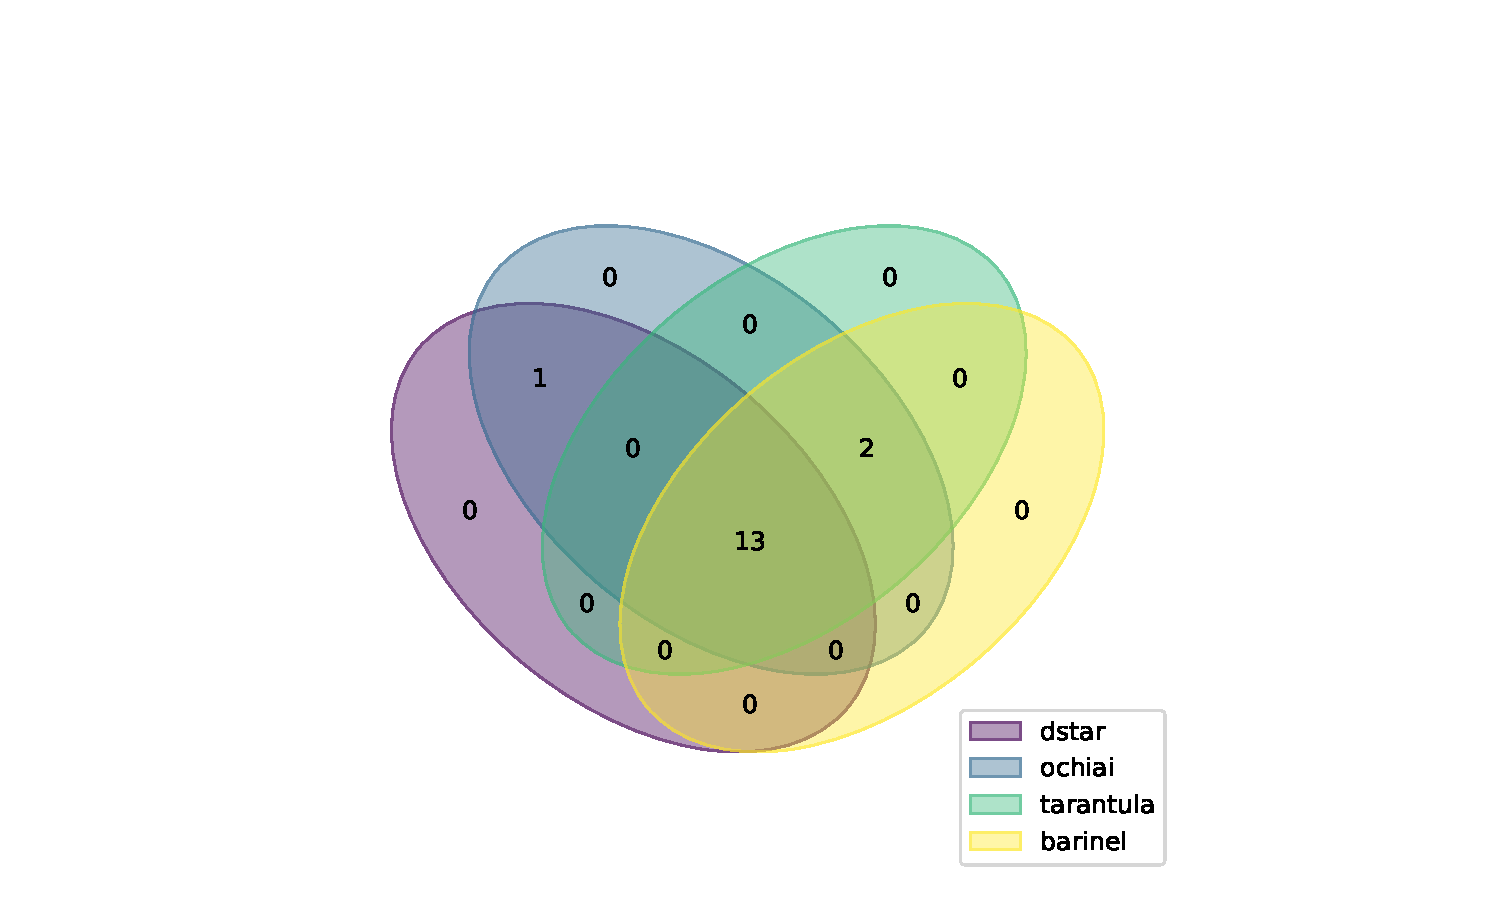
\includegraphics[width=0.35\textwidth, trim=40mm 0mm 40mm 30mm, clip]{figures/sherloc/venn_sbfls.pdf}
\vspace{-0.8em}
\caption{Venn-diagram of flaky classes ranked in the top 5 by the four SBFL \formulas.} 
% \centering}
\label{fig:sbfl_venn}
\vspace{-0.6em}
\end{figure}

\begin{tcolorbox}
% updated
Using SBFL, we were able to localise flaky classes by inspecting only 21-24\% (6-7\%) of classes covered by flaky tests on average (median). With Ochiai, flaky classes are ranked at the top and in the top 10 for 16\% and 55\% of total flaky commits. 
%Our results show that combining multiple Spectrum-Based Fault Localisation \formulas can rank 58\% of flaky classes in the top 10 and 13\% of them at the top.
\end{tcolorbox}

\subsection{RQ2 - Code and change metrics}
% JJ: to provide the reasoning or motivation for our usage of other data sources, such as static metrics and change history metrics. 

Table~\ref{tab:RQ2} shows the evaluation results for GP-evolved models using SBFL scores with change and code metrics.
The table shows that the addition of signals from change and size metrics leads to an improvement in the identification of flaky classes.
In particular, by adding change metrics, the percentage of classes ranked at the top reaches 24\%. 
This percentage is much higher than the maximum percentage achieved with SBFL alone, which is 16\% with Ochiai.
On the contrary, we do not observe any significant improvements in the number of flaky tests ranked in the top 10 or top 5. 
%Combined, these results imply that while these change and size metrics may not be effective alone, they can give additional signals that break ties between the classes located near the top, allowing developers to identify the exact cause of flakiness more precisely.
Combined, these results imply that these change and size metrics can give additional signals that break ties between the classes located near the top, allowing developers to identify the exact cause of flakiness more precisely.
The comparison with the results of GP with only SBFL \formulas in Table~\ref{tab:RQ1-GP} further supports the usefulness of change and size metrics.
Specifically, by adding change and size metrics, the percentage of flaky classes ranked at the top ($acc@1$) goes from 13\% to 24\% and 18\%, respectively. In addition, average $R_{wef}$ improves 5\% with change metrics and 4\% with size metrics. 

%That is the addition of flakiness and change metrics contributes only to a better ranking of classes at the top.
With regard to flakiness metrics, their combination with SBFL scores does not lead to any notable improvements in the ranking of classes at the top. 
The percentage of classes at the top is 11\% and the percentage of classes in the top 10 is 53\%.
One possible explanation for this is that our flakiness metrics are derived from a flakiness taxonomy that focuses on the test instead of the CUT.
%For instance, the most common category of flakiness, Asynchronous Waits, tend to appear in the test more than the CUT.
%This can be observed in the examples reported in the study of Luo~\etal~\cite{Luo2014}.
Hence, using metrics derived from such categories may not be helpful in the identification of CUT components that are responsible for flakiness.
To alleviate this, future studies should consider categories and metrics that are derived from the CUT, and existing flakiness taxonomies should be updated accordingly.
%Another potential reason behind this could be that the flakiness categories present in our dataset are different from the ones that we relied on. 
%In RQ4, we will further investigate this possibility.

\begin{table*}[ht]
\caption{RQ2: The contribution of flakiness, change, and size metrics to the identification of flaky classes. 
\label{tab:RQ2}\centering}
\centering
\scalebox{0.85}{
\begin{tabular}{c|rrrr|rr|rrrr|rr|rrrr|rr}
\toprule
& \multicolumn{6}{c|}{\textbf{SBFL \& flakiness}} & \multicolumn{6}{c|}{\textbf{SBFL \& change}} & \multicolumn{6}{c}{\textbf{SBFL \& size}}  \\
\textbf{Proj. (\#)} & \multicolumn{4}{c}{acc} & \multicolumn{2}{c|}{wef (R$_{wef}$)} & \multicolumn{4}{c}{acc} & \multicolumn{2}{c|}{wef (R$_{wef}$)} & \multicolumn{4}{c}{acc} & \multicolumn{2}{c}{wef (R$_{wef}$)}  \\
& @1 & @3 & @5 & @10 & mean & med & @1 & @3 & @5 & @10 & mean & med & @1 & @3 & @5 & @10 & mean & med \\
\midrule
%

Hbase (8) & 1 & 4 & 5 & 5 & 11.9 (12) & 3 (4) & 2 & 4 & 4 & 5 & 16.9 (13) & 4 (4) & 2 & 4 & 5 & 5 & 11.4 (12) & 3 (3) \\
Ignite (14) & 0 & 2 & 2 & 4 & 230.9 (26) & 63 (4) & 2 & 4 & 4 & 4 & 222.3 (24) & 18 (4) & 1 & 3 & 3 & 5 & 220.1 (24) & 43 (4) \\
Pulsar (10) & 2 & 5 & 6 & 8 & 10.2 (15) & 3 (8) & 3 & 5 & 7 & 9 & 8.0 (12) & 2 (5) & 2 & 5 & 7 & 9 & 6.9 (13) & 2 (6)  \\
Alluxio (3) & 0 & 0 & 1 & 1 & 97.7 (51) & 73 (65) & 0 & 0 & 1 & 1 & 75.7 (49) & 94 (39) & 0 & 0 & 1 & 1 & 90.7 (49) & 77 (58) \\
Neo4j (3) & 1 & 2 & 2 & 2 & 19.3 (42) & 1 (18) & 2 & 2 & 2 & 2 & 6.7 (37) & 0 (9) & 2 & 2 & 2 & 2 & 23.0 (40) & 0 (10) \\

\midrule
Total  (38) & 4 & 13 & 16 & 20 & 99.5 (24) & 8 (8) & 9 & 15 & 18 & 21 & 94.1 (21) & 5 (6) & 7 & 14 & 18 & 22 & 94.3 (22) & 5 (7) \\
Percentage (\%) & \textbf{11} & 34 & 42 & \textbf{53} & - & - & \textbf{24} & 39 & 47 & 55 & - & - & \textbf{18} & 37 & 47 & 58 & - & - \\

\bottomrule
\end{tabular}
}
\vspace{-4mm}
\end{table*}

%To further explain the positive contribution of change and flakiness metrics on the localisation performance, we analyse the effect of each additional metric on the GP evolved model.
To further investigate the impact of change and size metrics on the identification performance, we analyse the involvement of each metric in our GP-evolved \formulas. 
%Figures~\ref{fig:chg_metric_occur} and ~\ref{fig:flaky_metric_occur} show the frequency of change and size metrics in the GP evolved \formulas generated under (i) the configuration of using SBFL and change metrics and (ii) the configuration of using SBFL and size metrics, respectively. As shown in these figures, both change and size metrics are frequently involved in the final \formulas, confirming that our observed improvement did not come only from using GP.
Table~\ref{tab:RQ2-distr} shows the frequency of change and size metrics in the GP evolved \formulas generated under the configuration of using SBFL and change metrics (\ie SBFL \& Change) and the configuration of using SBFL and size metrics (\ie SBFL \& Size). 
As shown in this table, both change and size metrics are frequently involved in the final \formulas, confirming that our observed improvement did not come only from using GP.
Based on these results, we posit that change and size metrics can contribute positively to the identification of flaky classes. 

% Figure ~\ref{fig:chg_metric_occur} shows that \textsf{Age} is the change metric that appeared the most in the evolved \formulas.
% For flakiness metrics, we observe that concurrency (\textsf{\#COPS}), unordered collection (\textsf{\#UOPS}), and input/output (\textsf{\#IOPS}) are the metrics with the highest appearance frequency.
% On the other hand, random (\textsf{\#ROPS}) is the metric with the lowest appearance frequency and the metric of asynchronous waits (\textsf{\#AOPS}) does not have any contribution to the \formulas.

%\begin{figure}[t!]
%    \centering
%    \begin{subfigure}{0.35\textwidth}
%        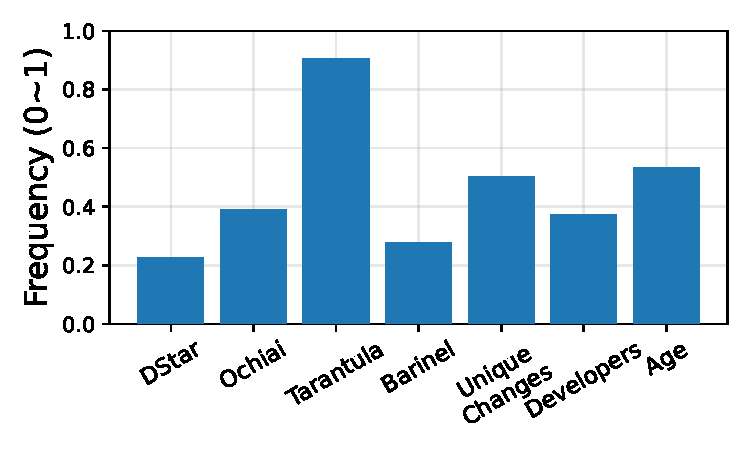
\includegraphics[width=\textwidth, trim=0mm 0mm 0mm 0mm, clip]{figures/sherloc/sbfl_chg_metric_occur.pdf}
%        \caption{The appearance of SBFL and change metrics in GP-evolved \formulas. \centering}
%        \label{fig:chg_metric_occur}
%    \end{subfigure}
%    \begin{subfigure}{0.35\textwidth}
%        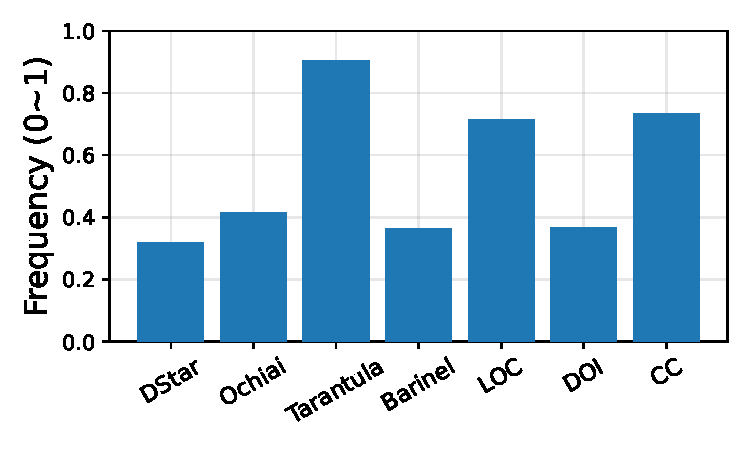
\includegraphics[width=\textwidth, trim=0mm 0mm 0mm 0mm, clip]{figures/sherloc/sbfl_size_metric_occur.pdf}
%        \caption{The appearance of SBFL and size metrics in GP-evolved \formulas. \centering}
%        \label{fig:flaky_metric_occur}
%    \end{subfigure}
%    \caption{Frequency of metrics in GP-evolved \formulas.\\
%    The y-axis denotes the ratio of \formulas that include each metric specified in the x-axis.\centering}
%    \label{fig:metric_appear_freq}
%\vspace{-4mm}
%\end{figure}

\begin{table}[ht]
\caption{Frequency of metrics in GP-evolved \formulas (from 0 to 1). `Changes' and `Dev' denote \textit{`Unique Changes'} and \textit{`Developers'}, respectively. The column `SBFL' contains the average frequency of the four SBFL metrics. 
\label{tab:RQ2-distr}}
\centering
\scalebox{0.85}{
\begin{tabular}{l|r|rrr|rrr}
\toprule
 & SBFL & Changes & Dev & Age & LOC & DOI & CC \\
\midrule
%SBFL &  & 0.23 & 0.39 & 0.91 & 0.28 & 0.50 & 0.37 & 0.53  & - & - & - \\
% & 0.32 & 0.42 & 0.90 & 0.36 & - & - & - & 0.71 & 0.37 & 0.73 \\
SBFL \& Change & 0.45 & 0.50 & 0.37 & 0.53  & - & - & - \\
SBFL \& Size & 0.50 & - & - & - & 0.71 & 0.37 & 0.73 \\
\bottomrule
\end{tabular}
}
\end{table}


\begin{tcolorbox}
%The augmentation of Spectrum-Based Fault Localisation with change and size metrics allows us to rank 24\% of flaky classes at the top. Nevertheless, metrics specific to flakiness categories do not provide any beneficial signals to the identification approach.
%The augmentation of Spectrum-Based Fault Localisation with change or size metrics leads to a better ranking of flaky classes near the top. 
The augmentation of Spectrum-Based Fault Localisation with change or size metrics lets more flaky classes be ranked near the top; by adding change metrics, we can rank 24\% flaky classes at the top. In contrast, metrics specific to flakiness categories do not provide any beneficial signals to the identification approach. 
\end{tcolorbox}

\subsection{RQ3 - Ensemble method}

% overall updated
Table~\ref{tab:RQ3-voting} presents the evaluation results for the voting method with 60 GP-evolved models, half from using SBFL and change metrics and the other half from using SBFL and size metrics.
%Half of the models use SBFL scores with change metrics, while the other half uses SBFL scores with size metrics. 
We decided to exclude the models that build on flakiness metrics since their usage did not improve the performance any further.
As explained in Section~\ref{sec:rq3_ensemble_method}, there can be a case where none of the participating models succeeds to vote for the true candidate since individual models vote only for those ranked within the top n. For this case, we report the median of all rankings of the models as an alternative. 

The results show that the voting step further improves the ranking results.
%Interestingly, the biggest improvements are in the accuracy in the top 5 and 3, which reach 53\% and 47\% respectively. At the top, the accuracy reaches 26\%, which is double the accuracy reached with GP-evolved models that rely solely on SBFL scores.In addition to the accuracy, the wasted effort with the voting method drops to 3.5, compared to 6.5 in models relying on SBFL scores.
The most notable improvement is the accuracy at the top 3, which reaches 47\%. Although the improvements in the other accuracy metrics are not as noticeable as what we have seen in the accuracy at the top 3, there are constant improvements over the results without voting. 
The average of wasted effort remains almost the same while the median improves from the voting, dropping to 3.5. These results imply that the voting allows those near the top to shift further to higher ranks based on the agreement among the models that exploit and capture different features of flaky classes.
Nonetheless, the constant improvements in $R_{we}$, both per project and in total, suggest that through the voting, we can rank flaky classes further near to the top; for example, in Alluxio, where $R_{wef}$ is always near 50, average $R_{wef}$ reduces to 22 and its median to 10. 
These results imply that voting can leverage the complementarity between different models, further improving the localisation of flakiness.
%Hence, we can deduce that voting between models based on SBFL, size, and change metrics provides the best ranking of flaky classes. \\

%As \textit{wef} only gives the absolute number of classes investigated before finding the flaky class, we wanted to balance this information with regards to the total number of classes covered by flaky tests. Accordingly, we also report, enclosed in parentheses in table~\ref{tab:RQ3-voting}, the average of wasted effort out of the total number of classes covered by flaky tests. 

\begin{table}[ht]
\caption{RQ3: The effectiveness of the voting between 60 different GP-evolved models, 30 from SBFL with change metrics, and 30 from using SBFL with size metrics. `Perc' denotes Percentage \label{tab:RQ3-voting}\centering}
\centering
\scalebox{0.9}{
\begin{tabular}{l|r|rrrr|rr}
\toprule
\textbf{Project} & \textbf{Total} & \multicolumn{4}{c|}{\textbf{acc}} & \multicolumn{2}{c}{\textbf{wef (R$_{wef}$)}} \\
& & @1 & @3 & @5 & @10 & mean & med \\
\midrule

Hbase & 8 & 3 & 5 & 6 & 6 & 9.62 (12) & 1.5 (2) \\
Ignite & 14 & 2 & 4 & 4 & 4 & 228.61 (24) & 17.5 (4) \\
Pulsar & 10 & 3 & 6 & 7 & 9 & 7.30 (12) & 2.0 (5) \\
Alluxio & 3 & 1 & 1 & 1 & 2 & 61.83 (22) & 9.0 (10) \\
Neo4j & 3 & 1 & 2 & 2 & 2 & 19.67 (42) & 1.0 (18) \\

\midrule
Total & 38 & 10 & 18 & 20 & 23 & 94.61 (19) & 3.5 (5) \\
Perc (\%) & 100 & 26 & \textbf{47} & 53 & 61 & - & - \\

\bottomrule
\end{tabular}
}
\vspace{-4mm}
\end{table}

% \textbf{
% \begin{figure}[ht]
% \centering
% 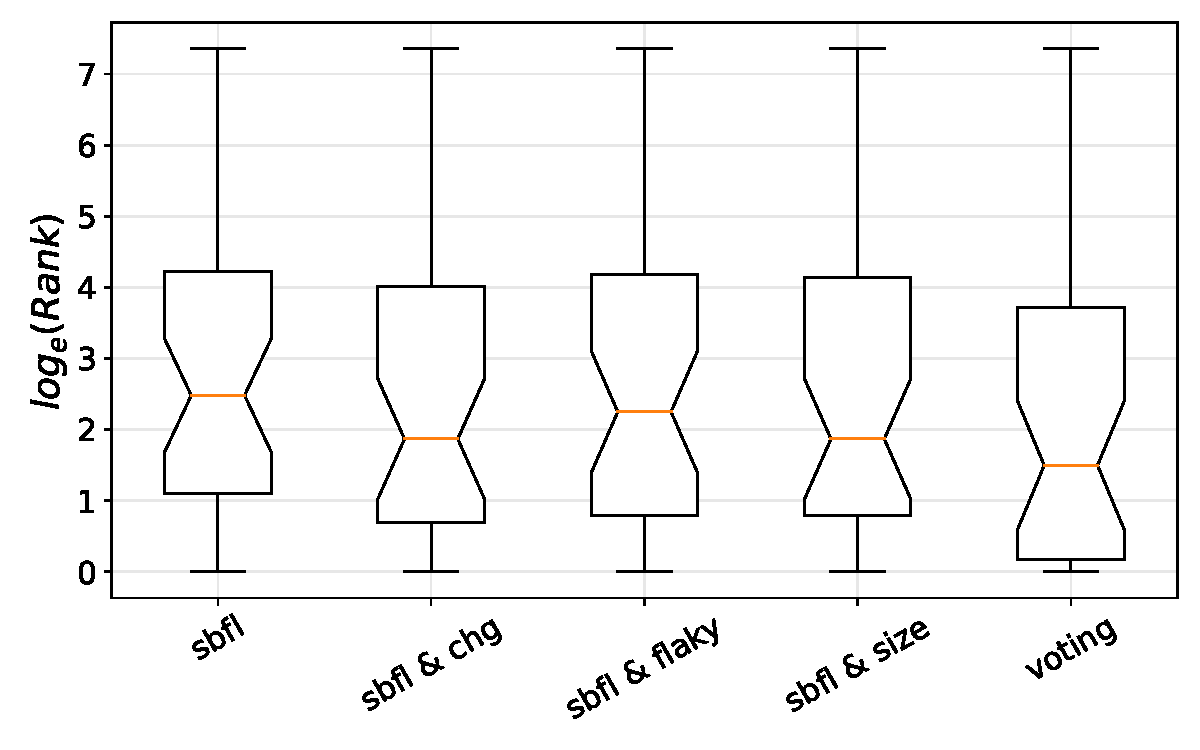
\includegraphics[width=75mm]{figures/sherloc/rank_distr_final.pdf}
% \caption{Distribution of flaky class ranking with the different SBFL-based approaches}
% \label{fig:rank}
% \end{figure}}

\begin{tcolorbox}
A voting between models based on SBFL, change, and size metrics, provides the best ranking for flaky classes.
47\% of flaky classes are ranked in the top 3 and 26\% of them are ranked at the top. The average $R_{wef}$ further reduces to 19, highlighting the practical usefulness of our approach.  
\end{tcolorbox}

\subsection{RQ4 - Flakiness categories}
Table~\ref{tab:RQ4} presents the performances of the voting method on the different flakiness categories encountered in our dataset.
The \textit{``Ambiguous"} category represents cases where the flaky tests could not be assigned to any of the known flakiness categories.
First, we observe that the most common categories are Concurrency and Asynchronous Waits.
This aligns with observations from previous studies~\cite{Luo2014,Lam2020a,Eck2019} and confirms that the taxonomy adopted for our metrics is adequate for our distribution.
Furthermore, we observe a discrepancy between the performances in different categories.
Classes responsible for Async Waits are well identified with 80\% of the classes in the top 10, and 30\% of them at the top.
Classes responsible for Concurrency also show good performances with 50\% of them in the top 10, and 38\% of them at the top; the average $R_{wef}$ is below ten, eight precisely, meaning we can locate flaky classes by inspecting less than 10\% of the total number of the classes covered by flaky tests. 

Categories such as Time and I/O show much lower performances, with 33\% and 0\% of flaky classes in the top 10, respectively.
Nevertheless, given the low number of instances for these categories, it is hard to discuss or generalise their results.
With only two instances, the category Unordered Collections shows curious results as one class is ranked second and the other one ranked 663. 
To understand the reasons behind the bad ranking, we manually inspected this case\footnote{\url{https://github.com/apache/ignite/commit/188e4d52c2}}.  
We found that the concerned test, \texttt{testUnstableTopology}, was executed twice due to a retry mechanism. Both executions led to failure, but interestingly, we found that the two failures have different causes. One of them is due to a lack of context initialisation and is likely to be the reason behind flakiness. 
As the two failure causes are different, the coverage is also different in them.
Specifically, one of the failures  did not cover the flaky class, and as the coverage of this failure was leveraged in the SBFL, the flaky class was not considered suspicious.
We discuss other reasons responsible for poor ranking in Section~\ref{sec:discussion}.
%To conclude this section that the performances of the SBFL-based approach differ considerably between different flakiness categories.


% "Hard to classify" changed to "Ambiguous"
\begin{table}[ht]
\caption{RQ4: The effectiveness per flakiness category \label{tab:RQ4}\centering}
\centering
\scalebox{0.8}{
\begin{tabular}{l|cccc|cc}
\toprule
\textbf{Flakiness} & \multicolumn{4}{c|}{\textbf{acc}} & \multicolumn{2}{c}{\textbf{wef (R$_{wef}$)}} \\
\textbf{Category} & @1 & @3 & @5 & @10 & mean & med \\
\midrule

Concurrency (16) & 6 (\textbf{38}) & 7 (44) & 7(44) & 8 (\textbf{50})& 147.53 (27) & 9.5 (9) \\
Async wait (10) & 3 (\textbf{30}) & 6 (60) & 8 (80) & 8 (\textbf{80})& 21.05 (8) & 1.5 (3) \\ 

Ambiguous (4) & 1 (25) & 2 (50) & 2 (50) & 3 (75)& 18.88 (5) & 3.5 (5) \\
Time (3) & 0 (0) & 0 (0) & 0 (0) & 1 (\textbf{33})& 88.33 (16) & 14.0 (10) \\
Network (2) & 0 (0) & 2 (100) & 2 (100) & 2 (100)& 1.00 (10) & 1.0 (10) \\
Unordered  &  &  &  &  & &  \\
collections (2) & 0 (0) & 1 (50) & 1(50) & 1 (50) & 331.5 (33) & 331.5 (33) \\
I/O (1) & 0 (0) & 0 (0) & 0(0) & 0 (\textbf{0})& 12.50 (3) & 12.5 (3) \\
Random (1) & 0 (0) & 1 (100) & 1 (100) & 1 (100)& 2.00 (75) & 2.0 (75) \\

%Network &  &  &  &  & &  \\
%Unordered (1) & 0 (0) & 1 (100) & 1(100) & 1 (100)& 1.00 & 1.0 \\
%collections &  &  &  &  & &  \\

\midrule
Total (39\tablefootnote{One flaky class belongs to two categories: Network and Unordered Collections.}) & 10 & 18 & 20 & 23 & 94.47 (19) & 3.5 (5) \\
Perc (\%) & 26 & 47 & 53 & 61 & - & - \\

\bottomrule
\end{tabular}
}
\vspace{-4mm}
\end{table}

\begin{tcolorbox}
The most prominent flakiness categories, Concurrency and Asynchronous Waits, are identified effectively, with 38\%
and 30\% of their flaky classes ranked at the top, respectively.
In the Concurrency category, flaky classes are identified by examining 8\% of classes covered by flaky tests on average. 
\end{tcolorbox}